\documentclass[10pt,onecolumn]{article}

\usepackage{graphicx}
\usepackage{hyperref}
\usepackage{xcolor}
\hypersetup{
  colorlinks = true,
  citecolor  = red
}

\begin{document}

\title{Communicating between the kernel and user-space in Linux using Netlink Sockets}
\author{}
\date{}
\maketitle

\section{NETLINK SOCKETS}
\subsection{What is Netlink?}
Netlink is a datagram-oriented messaging system that allows passing messages from kernel to user-space and vice-versa.

Netlink is implemented on top of the generic BSD socket infrastructure, thus, it supports usual primitives like \textit{socket}(), \textit{bind}(), \textit{sendmsg}() and \textit{recvmsg}() as well as common socket polling mechanisms.

\subsection{Netlink socket bus}
Netlink allows up to 32 buses in kernel-space, where each bus deals with a specific service; for example, different Netlink busses exist for routing (NETLINK\_ROUTE), netfilter (eg, NETLINK\_NETFILTER), and several other kernel subsystems.

\subsection{Netlink message format}

\begin{figure}[h]
\begin{center}
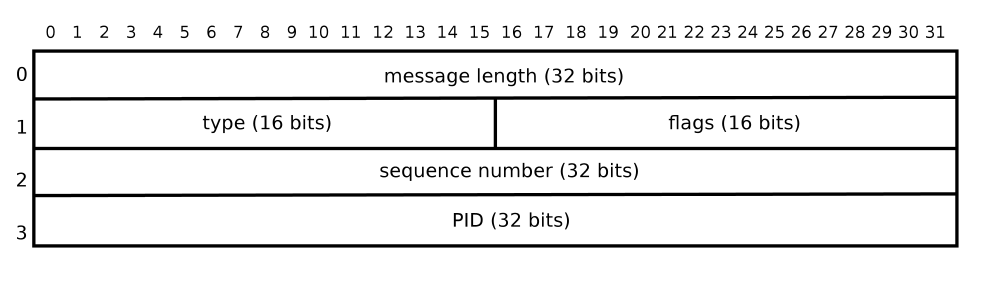
\includegraphics[height=3cm]{figure/netlink_message_header.png}
\end{center}
\caption{Layout of a Netlink message header}
\label{fig:netlink_message_header}
\end{figure}

A Netlink message always starts by a fixed header of 16 bytes defined by \textit{struct nlmsghdr} in \textit{\textless include/linux/netlink.h \textgreater}. We have represented this header in Figure \ref{fig:netlink_message_header}. This header contains the following fields:

\begin{itemize}
\item Message length (32 bits): size of the message in bytes, including this header.
\item Message type (16 bits): the type of the message. There are two sorts, data and control messages. Data messages depend on the set of actions that the given kernel-space subsystem allows. Control messages are common to all Netlink subsystems, there are currently four types of control messages, although there are 16 slots reserved. The existing control types are:
  \begin{itemize}
  \item NLMSG\_NOOP: no operation, this can be used to implement a Netlink ping utility to know if a given Netlink bus is available.
  \end{itemize}
\item Message flags (16 bits): several message flags like:
  \begin{itemize}
  \item NLM\_F\_REQUEST: if this flag is set, this Netlink message contains a request. Messages that go from user to kernel-space must set this flag, otherwise the kernel subsystem must report an \textit{invalid argument} (EINVAL) error to the user-space sender.
  \item NLM\_F\_ACK: the user-space application requested a confirmation message from kernel-space to make sure that a given request was successfully performed.
  \item ...
  \end{itemize}
\item Sequence number (32 bits): message sequence number. This is useful together with NLM\_F\_ACK if an user-space application wants to make sure that a request has been correctly issued. Netlink uses the same sequence number in the message that are sent as reply to a given request.
\item Port-ID (32 bits): this field contains a numerical identifier that is assigned by Netlink. Netlink assigns different port-ID values to identify several socket channels opened by the same user-space.
\end{itemize}

The payload of Netlink messages is compose of a set of attributes that are expressed in Type-Length-Value (TLV) format. Each Netlink attribute header is defined by \textit{struct nlattr} and is composed of the following fields:

\begin{itemize}
\item Type (16 bits): the attribute type according to the set of available types in the kernel subsystem. The two most significant bits of this field are used to encode if this is a nested attribute (bit 0), which allows you to embed a set of attributes in the payload of one attribute, and if the attribute payload is represented in network byte order (bit 1).
\item Length (16 bits): size in bytes of the attribute. This includes this header header plus the payload size of this attribute without alignment to 32 bits.
\item Value: this field is variable in size but it is always aligned to 32 bits.
\end{itemize}

\begin{figure}[h]
\begin{center}
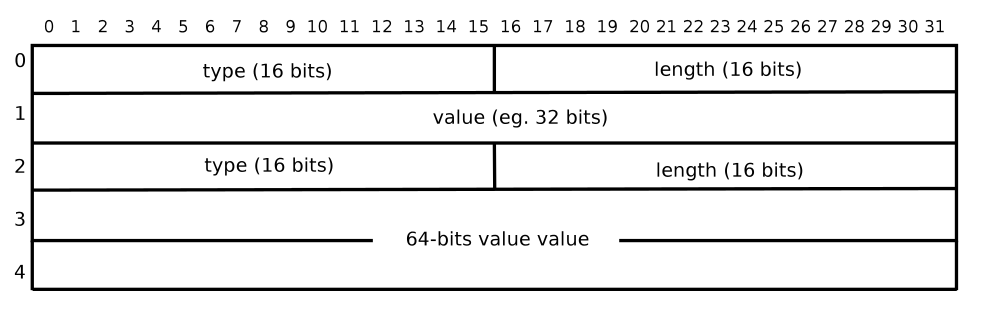
\includegraphics[height=3cm]{figure/netlink_payload.png}
\end{center}
\caption{An example of a hypothetical Netlink payload in TLV format}
\label{fig:netlink_payload}
\end{figure}

In Figure. \ref{fig:netlink_payload} we have represented a hypothetical payload in TLV format composed on two attributes, one of 32 bits and another of 64 bits.

Another interesting feature of Netlink is attribute nesting that allows you to embed a set of attributes in the payload of one single attribute. For example, if you have a traffic-flow object that you have to expose to user-space via Netlink, the object's layer 3 address can be in IPv4 (32 bits) or IPv6 (128-bits) format, assuming that the system supports both IPv4 and IPv6 at the same time.

\begin{figure}[h]
\begin{center}
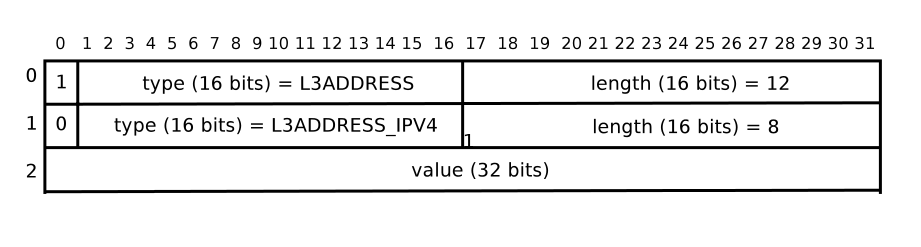
\includegraphics[height=3cm]{figure/netlink_nested_attribute.png}
\end{center}
\caption{Example of a nested attribute}
\label{fig:netlink_nested_attribute}
\end{figure}

In Figure. \ref{fig:netlink_nested_attribute}, we have represented an example in which we have defined a generic attribute L3ADDRESS that may contain a set of attributes like L3ADDRESS\_IPV4 and L3ADDRESS\_IPV6. The attributes L3ADDRESS\_IPV4 and L3ADDRESS\_IPV6 can be used to encapsulate the specific address information. Thus, in the particular case of an IPv4 traffic-flow, L3ADDRESS encapsulates L3ADDRESS\_IPV4 attributes. Moreover, if we want to add support for a new layer 3 protocol, eg. Internetwork Packet Exchange (IPX), we only have to add the new attribute.

\section{GENETLINK: GENERIC NETLINK MULTIPLEXATION}

GeNetlink, or Generic Netlink, is a multiplexer that is built on top of a Netlink bus (NETLINK\_GENERIC) and was introduced during the 2.6.15 development cycle. Over the years, Netlink has becomes very popular, this has brought about a real concern that the number Netlink buses may be exhausted in the near future. In response to this the Generic Netlink was created.

GeNetlink allows to register up to 65520 families that share a single Netlink bus. Each family is intended to be equivalent to a virtual bus. The families that are registered in GeNetlink are identified by a unique string name and ID number.

When GeNetlink is loaded, it initially registers a control family, the so-called \textit{nlctrl}, that provides a lookup facility to obtain the ID number from the string name that identifies families, and event reports to inform about the registration and unregistration of new GeNetlink services and its features. The control family is the only GeNetlink service that has a fixed ID number (GENL\_ID\_CTRL which is equal to 16) while the vast majority of other families use a system-dependant ID number that is assigned in run-time.

GeNetlink families can also register multicast groups. In this case, the multicast groups are identified by a unique string name that remains the primary key. During the registration of the multicast group, a unique ID number for that group is set.

\subsection{GeNetlink message format}

GeNetlink messages start by the Netlink header, whose message type is the ID number of the GeNetlink service, then it follows the GeNetlink header and finally one optional header that is specific of the given GeNetlink service. Thus, GeNetlink messages may contain up to three headers before the TLV-based payload. Since the ID number of the service is required to build the GeNetlink message, GeNetlink provides a lookup facility to resolve the ID number from the service string name. We have represented the GeNetlink header in Figure. \ref{fig:genetlink_message_header}.

\begin{figure}[h]
\begin{center}
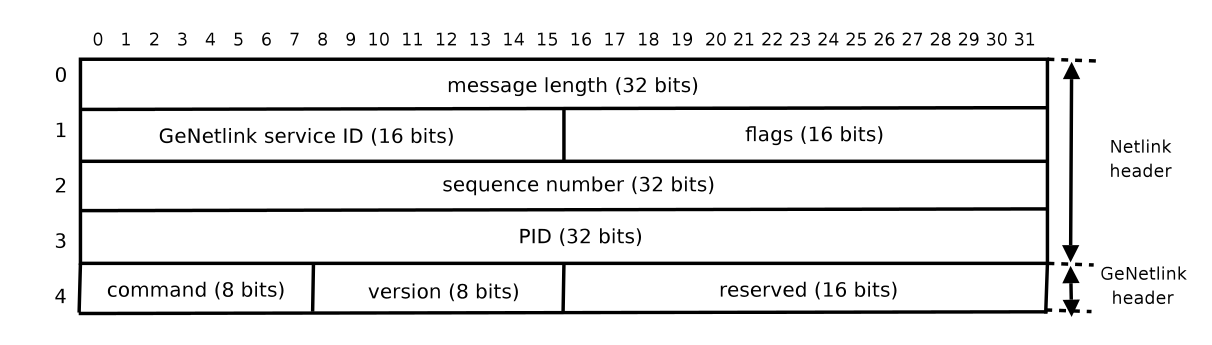
\includegraphics[height=3cm]{figure/genetlink_message_header.png}
\end{center}
\caption{Layout of a GeNetlink header message}
\label{fig:genetlink_message_header}
\end{figure}

The GeNetlink header contains three fields:

\begin{itemize}
  \item The \textit{command} field (8 bits), that is a specific message type of the GeNetlink service.
\end{itemize}

\subsection{GeNetlink control family}

The GeNetlink control family \textit{nlctrl} provides the following commands to user-space applications:

\begin{itemize}
  \item CTRL\_CMD\_GETFAMILY: this command allows to look up for the family ID number from the family name.
\end{itemize}

Since the family and multicast IDs are assigned in run-time, we initially have to look up for the IDs to send requests and to subscribe to GeNetlink multicast groups from user-space. For that task, the user-space application sends a CTRL\_CMD\_GETFAMILY request to the GeNetlink control family. Then, once it receives the look-up response that contains the family ID number, the supported operations and the existing multicast groups; the user-space application can build the message for the specific GeNetlink family subsystem to request some operation. The message payload must also contain the mandatory attributes for that operation.

\section{PROGRAMMING NETLINK SOCKETS}

In order to simplify the work with Netlink sockets in user-space, we propose the use of user-space libraries such as \textit{libnl} and \textit{libmnl}. These libraries are written in C and that are targeted to Netlink developers.

\end{document}
